\documentclass[1p]{elsarticle_modified}
%\bibliographystyle{elsarticle-num}

%\usepackage[colorlinks]{hyperref}
%\usepackage{abbrmath_seonhwa} %\Abb, \Ascr, \Acal ,\Abf, \Afrak
\usepackage{amsfonts}
\usepackage{amssymb}
\usepackage{amsmath}
\usepackage{amsthm}
\usepackage{scalefnt}
\usepackage{amsbsy}
\usepackage{kotex}
\usepackage{caption}
\usepackage{subfig}
\usepackage{color}
\usepackage{graphicx}
\usepackage{xcolor} %% white, black, red, green, blue, cyan, magenta, yellow
\usepackage{float}
\usepackage{setspace}
\usepackage{hyperref}

\usepackage{tikz}
\usetikzlibrary{arrows}

\usepackage{multirow}
\usepackage{array} % fixed length table
\usepackage{hhline}

%%%%%%%%%%%%%%%%%%%%%
\makeatletter
\renewcommand*\env@matrix[1][\arraystretch]{%
	\edef\arraystretch{#1}%
	\hskip -\arraycolsep
	\let\@ifnextchar\new@ifnextchar
	\array{*\c@MaxMatrixCols c}}
\makeatother %https://tex.stackexchange.com/questions/14071/how-can-i-increase-the-line-spacing-in-a-matrix
%%%%%%%%%%%%%%%

\usepackage[normalem]{ulem}

\newcommand{\msout}[1]{\ifmmode\text{\sout{\ensuremath{#1}}}\else\sout{#1}\fi}
%SOURCE: \msout is \stkout macro in https://tex.stackexchange.com/questions/20609/strikeout-in-math-mode

\newcommand{\cancel}[1]{
	\ifmmode
	{\color{red}\msout{#1}}
	\else
	{\color{red}\sout{#1}}
	\fi
}

\newcommand{\add}[1]{
	{\color{blue}\uwave{#1}}
}

\newcommand{\replace}[2]{
	\ifmmode
	{\color{red}\msout{#1}}{\color{blue}\uwave{#2}}
	\else
	{\color{red}\sout{#1}}{\color{blue}\uwave{#2}}
	\fi
}

\newcommand{\Sol}{\mathcal{S}} %segment
\newcommand{\D}{D} %diagram
\newcommand{\A}{\mathcal{A}} %arc


%%%%%%%%%%%%%%%%%%%%%%%%%%%%%5 test

\def\sl{\operatorname{\textup{SL}}(2,\Cbb)}
\def\psl{\operatorname{\textup{PSL}}(2,\Cbb)}
\def\quan{\mkern 1mu \triangleright \mkern 1mu}

\theoremstyle{definition}
\newtheorem{thm}{Theorem}[section]
\newtheorem{prop}[thm]{Proposition}
\newtheorem{lem}[thm]{Lemma}
\newtheorem{ques}[thm]{Question}
\newtheorem{cor}[thm]{Corollary}
\newtheorem{defn}[thm]{Definition}
\newtheorem{exam}[thm]{Example}
\newtheorem{rmk}[thm]{Remark}
\newtheorem{alg}[thm]{Algorithm}

\newcommand{\I}{\sqrt{-1}}
\begin{document}

%\begin{frontmatter}
%
%\title{Boundary parabolic representations of knots up to 8 crossings}
%
%%% Group authors per affiliation:
%\author{Yunhi Cho} 
%\address{Department of Mathematics, University of Seoul, Seoul, Korea}
%\ead{yhcho@uos.ac.kr}
%
%
%\author{Seonhwa Kim} %\fnref{s_kim}}
%\address{Center for Geometry and Physics, Institute for Basic Science, Pohang, 37673, Korea}
%\ead{ryeona17@ibs.re.kr}
%
%\author{Hyuk Kim}
%\address{Department of Mathematical Sciences, Seoul National University, Seoul 08826, Korea}
%\ead{hyukkim@snu.ac.kr}
%
%\author{Seokbeom Yoon}
%\address{Department of Mathematical Sciences, Seoul National University, Seoul, 08826,  Korea}
%\ead{sbyoon15@snu.ac.kr}
%
%\begin{abstract}
%We find all boundary parabolic representation of knots up to 8 crossings.
%
%\end{abstract}
%\begin{keyword}
%    \MSC[2010] 57M25 
%\end{keyword}
%
%\end{frontmatter}

%\linenumbers
%\tableofcontents
%
\newcommand\colored[1]{\textcolor{white}{\rule[-0.35ex]{0.8em}{1.4ex}}\kern-0.8em\color{red} #1}%
%\newcommand\colored[1]{\textcolor{white}{ #1}\kern-2.17ex	\textcolor{white}{ #1}\kern-1.81ex	\textcolor{white}{ #1}\kern-2.15ex\color{red}#1	}

{\Large $\underline{12n_{0684}~(K12n_{0684})}$}

\setlength{\tabcolsep}{10pt}
\renewcommand{\arraystretch}{1.6}
\vspace{1cm}\begin{tabular}{m{100pt}>{\centering\arraybackslash}m{274pt}}
\multirow{5}{120pt}{
	\centering
	\includegraphics[width=112pt]{../../../GIT/diagram.site/Diagrams/png/2773_12n_0684.png}\\
\ \ \ A knot diagram\footnotemark}&
\allowdisplaybreaks
\textbf{Linearized knot diagam} \\
\cline{2-2}
 &
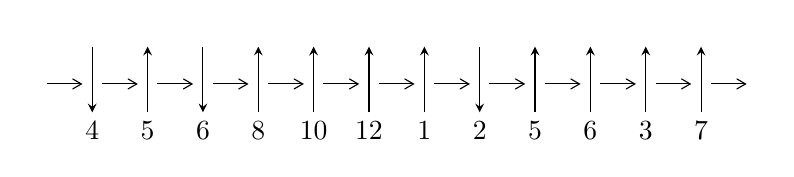
\begin{tikzpicture}[x=20pt, y=17pt]
	% nodes
	\node (C0) at (0, 0) {};
	\node (C1) at (1, 0) {};
	\node (C1U) at (1, +1) {};
	\node (C1D) at (1, -1) {4};

	\node (C2) at (2, 0) {};
	\node (C2U) at (2, +1) {};
	\node (C2D) at (2, -1) {5};

	\node (C3) at (3, 0) {};
	\node (C3U) at (3, +1) {};
	\node (C3D) at (3, -1) {6};

	\node (C4) at (4, 0) {};
	\node (C4U) at (4, +1) {};
	\node (C4D) at (4, -1) {8};

	\node (C5) at (5, 0) {};
	\node (C5U) at (5, +1) {};
	\node (C5D) at (5, -1) {10};

	\node (C6) at (6, 0) {};
	\node (C6U) at (6, +1) {};
	\node (C6D) at (6, -1) {12};

	\node (C7) at (7, 0) {};
	\node (C7U) at (7, +1) {};
	\node (C7D) at (7, -1) {1};

	\node (C8) at (8, 0) {};
	\node (C8U) at (8, +1) {};
	\node (C8D) at (8, -1) {2};

	\node (C9) at (9, 0) {};
	\node (C9U) at (9, +1) {};
	\node (C9D) at (9, -1) {5};

	\node (C10) at (10, 0) {};
	\node (C10U) at (10, +1) {};
	\node (C10D) at (10, -1) {6};

	\node (C11) at (11, 0) {};
	\node (C11U) at (11, +1) {};
	\node (C11D) at (11, -1) {3};

	\node (C12) at (12, 0) {};
	\node (C12U) at (12, +1) {};
	\node (C12D) at (12, -1) {7};
	\node (C13) at (13, 0) {};

	% arrows
	\draw[->,>={angle 60}]
	(C0) edge (C1) (C1) edge (C2) (C2) edge (C3) (C3) edge (C4) (C4) edge (C5) (C5) edge (C6) (C6) edge (C7) (C7) edge (C8) (C8) edge (C9) (C9) edge (C10) (C10) edge (C11) (C11) edge (C12) (C12) edge (C13) ;	\draw[->,>=stealth]
	(C1U) edge (C1D) (C2D) edge (C2U) (C3U) edge (C3D) (C4D) edge (C4U) (C5D) edge (C5U) (C6D) edge (C6U) (C7D) edge (C7U) (C8U) edge (C8D) (C9D) edge (C9U) (C10D) edge (C10U) (C11D) edge (C11U) (C12D) edge (C12U) ;
	\end{tikzpicture} \\
\hhline{~~} \\& 
\textbf{Solving Sequence} \\ \cline{2-2} 
 &
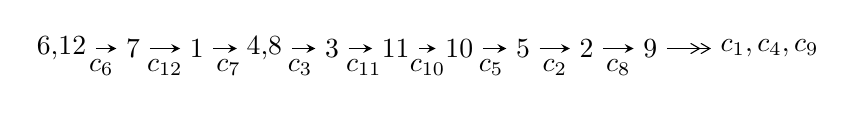
\begin{tikzpicture}[x=23pt, y=7pt]
	% node
	\node (A0) at (-1/8, 0) {6,12};
	\node (A1) at (1, 0) {7};
	\node (A2) at (2, 0) {1};
	\node (A3) at (49/16, 0) {4,8};
	\node (A4) at (33/8, 0) {3};
	\node (A5) at (41/8, 0) {11};
	\node (A6) at (49/8, 0) {10};
	\node (A7) at (57/8, 0) {5};
	\node (A8) at (65/8, 0) {2};
	\node (A9) at (73/8, 0) {9};
	\node (C1) at (1/2, -1) {$c_{6}$};
	\node (C2) at (3/2, -1) {$c_{12}$};
	\node (C3) at (5/2, -1) {$c_{7}$};
	\node (C4) at (29/8, -1) {$c_{3}$};
	\node (C5) at (37/8, -1) {$c_{11}$};
	\node (C6) at (45/8, -1) {$c_{10}$};
	\node (C7) at (53/8, -1) {$c_{5}$};
	\node (C8) at (61/8, -1) {$c_{2}$};
	\node (C9) at (69/8, -1) {$c_{8}$};
	\node (A10) at (11, 0) {$c_{1},c_{4},c_{9}$};

	% edge
	\draw[->,>=stealth]	
	(A0) edge (A1) (A1) edge (A2) (A2) edge (A3) (A3) edge (A4) (A4) edge (A5) (A5) edge (A6) (A6) edge (A7) (A7) edge (A8) (A8) edge (A9) ;
	\draw[->>,>={angle 60}]	
	(A9) edge (A10);
\end{tikzpicture} \\ 

\end{tabular} \\

\footnotetext{
The image of knot diagram is generated by the software ``\textbf{Draw programme}" developed by Andrew Bartholomew(\url{http://www.layer8.co.uk/maths/draw/index.htm\#Running-draw}), where we modified some parts for our purpose(\url{https://github.com/CATsTAILs/LinksPainter}).
}\phantom \\ \newline 
\centering \textbf{Ideals for irreducible components\footnotemark of $X_{\text{par}}$} 
 
\begin{align*}
I^u_{1}&=\langle 
2.79905\times10^{36} u^{48}-3.47735\times10^{36} u^{47}+\cdots+2.46397\times10^{35} b-8.54140\times10^{36},\\
\phantom{I^u_{1}}&\phantom{= \langle  }-1.52263\times10^{37} u^{48}+2.01595\times10^{37} u^{47}+\cdots+2.46397\times10^{35} a+4.41343\times10^{37},\;u^{49}- u^{48}+\cdots-11 u-1\rangle \\
I^u_{2}&=\langle 
u^8-6 u^6- u^5+11 u^4+4 u^3-6 u^2+b-3 u,\\
\phantom{I^u_{2}}&\phantom{= \langle  }- u^9- u^8+7 u^7+7 u^6-16 u^5-16 u^4+13 u^3+13 u^2+a-3 u-2,\\
\phantom{I^u_{2}}&\phantom{= \langle  }u^{11}-8 u^9- u^8+23 u^7+6 u^6-28 u^5-11 u^4+12 u^3+6 u^2-1\rangle \\
\\
\end{align*}
\raggedright * 2 irreducible components of $\dim_{\mathbb{C}}=0$, with total 60 representations.\\
\footnotetext{All coefficients of polynomials are rational numbers. But the coefficients are sometimes approximated in decimal forms when there is not enough margin.}
\newpage
\renewcommand{\arraystretch}{1}
\centering \section*{I. $I^u_{1}= \langle 2.80\times10^{36} u^{48}-3.48\times10^{36} u^{47}+\cdots+2.46\times10^{35} b-8.54\times10^{36},\;-1.52\times10^{37} u^{48}+2.02\times10^{37} u^{47}+\cdots+2.46\times10^{35} a+4.41\times10^{37},\;u^{49}- u^{48}+\cdots-11 u-1 \rangle$}
\flushleft \textbf{(i) Arc colorings}\\
\begin{tabular}{m{7pt} m{180pt} m{7pt} m{180pt} }
\flushright $a_{6}=$&$\begin{pmatrix}1\\0\end{pmatrix}$ \\
\flushright $a_{12}=$&$\begin{pmatrix}0\\u\end{pmatrix}$ \\
\flushright $a_{7}=$&$\begin{pmatrix}1\\- u^2\end{pmatrix}$ \\
\flushright $a_{1}=$&$\begin{pmatrix}u\\- u^3+u\end{pmatrix}$ \\
\flushright $a_{4}=$&$\begin{pmatrix}61.7957 u^{48}-81.8168 u^{47}+\cdots-1478.08 u-179.118\\-11.3599 u^{48}+14.1128 u^{47}+\cdots+260.816 u+34.6651\end{pmatrix}$ \\
\flushright $a_{8}=$&$\begin{pmatrix}- u^2+1\\u^4-2 u^2\end{pmatrix}$ \\
\flushright $a_{3}=$&$\begin{pmatrix}50.4358 u^{48}-67.7041 u^{47}+\cdots-1217.27 u-144.453\\-11.3599 u^{48}+14.1128 u^{47}+\cdots+260.816 u+34.6651\end{pmatrix}$ \\
\flushright $a_{11}=$&$\begin{pmatrix}0.0440751 u^{48}+0.409727 u^{47}+\cdots+27.7427 u+11.4620\\-14.3871 u^{48}+19.4508 u^{47}+\cdots+353.858 u+45.6249\end{pmatrix}$ \\
\flushright $a_{10}=$&$\begin{pmatrix}14.4312 u^{48}-19.0411 u^{47}+\cdots-326.115 u-34.1629\\-14.3871 u^{48}+19.4508 u^{47}+\cdots+353.858 u+45.6249\end{pmatrix}$ \\
\flushright $a_{5}=$&$\begin{pmatrix}64.0525 u^{48}-85.7056 u^{47}+\cdots-1545.71 u-185.562\\-12.0629 u^{48}+15.1894 u^{47}+\cdots+279.471 u+36.8940\end{pmatrix}$ \\
\flushright $a_{2}=$&$\begin{pmatrix}49.9570 u^{48}-67.3760 u^{47}+\cdots-1201.28 u-146.399\\-23.5956 u^{48}+30.8548 u^{47}+\cdots+561.583 u+71.2213\end{pmatrix}$ \\
\flushright $a_{9}=$&$\begin{pmatrix}4.08898 u^{48}-6.07759 u^{47}+\cdots-126.997 u-13.5152\\20.0723 u^{48}-26.3130 u^{47}+\cdots-472.737 u-58.6870\end{pmatrix}$\\&\end{tabular}
\flushleft \textbf{(ii) Obstruction class $= -1$}\\~\\
\flushleft \textbf{(iii) Cusp Shapes $= 16.0931 u^{48}-20.2673 u^{47}+\cdots-400.029 u-58.9748$}\\~\\
\newpage\renewcommand{\arraystretch}{1}
\flushleft \textbf{(iv) u-Polynomials at the component}\newline \\
\begin{tabular}{m{50pt}|m{274pt}}
Crossings & \hspace{64pt}u-Polynomials at each crossing \\
\hline $$\begin{aligned}c_{1}\end{aligned}$$&$\begin{aligned}
&u^{49}+u^{48}+\cdots+25 u-7
\end{aligned}$\\
\hline $$\begin{aligned}c_{2}\end{aligned}$$&$\begin{aligned}
&u^{49}+2 u^{48}+\cdots-33 u+1
\end{aligned}$\\
\hline $$\begin{aligned}c_{3}\end{aligned}$$&$\begin{aligned}
&u^{49}-3 u^{48}+\cdots+210 u-19
\end{aligned}$\\
\hline $$\begin{aligned}c_{4}\end{aligned}$$&$\begin{aligned}
&u^{49}-9 u^{47}+\cdots-36 u+8
\end{aligned}$\\
\hline $$\begin{aligned}c_{5},c_{9},c_{10}\end{aligned}$$&$\begin{aligned}
&u^{49}+u^{48}+\cdots-13 u+1
\end{aligned}$\\
\hline $$\begin{aligned}c_{6},c_{7},c_{12}\end{aligned}$$&$\begin{aligned}
&u^{49}- u^{48}+\cdots-11 u-1
\end{aligned}$\\
\hline $$\begin{aligned}c_{8}\end{aligned}$$&$\begin{aligned}
&u^{49}-20 u^{47}+\cdots+8 u-1
\end{aligned}$\\
\hline $$\begin{aligned}c_{11}\end{aligned}$$&$\begin{aligned}
&u^{49}-3 u^{48}+\cdots+288 u-32
\end{aligned}$\\
\hline
\end{tabular}\\~\\
\newpage\renewcommand{\arraystretch}{1}
\flushleft \textbf{(v) Riley Polynomials at the component}\newline \\
\begin{tabular}{m{50pt}|m{274pt}}
Crossings & \hspace{64pt}Riley Polynomials at each crossing \\
\hline $$\begin{aligned}c_{1}\end{aligned}$$&$\begin{aligned}
&y^{49}-5 y^{48}+\cdots+4153 y-49
\end{aligned}$\\
\hline $$\begin{aligned}c_{2}\end{aligned}$$&$\begin{aligned}
&y^{49}+48 y^{48}+\cdots+37 y-1
\end{aligned}$\\
\hline $$\begin{aligned}c_{3}\end{aligned}$$&$\begin{aligned}
&y^{49}-35 y^{48}+\cdots+18032 y-361
\end{aligned}$\\
\hline $$\begin{aligned}c_{4}\end{aligned}$$&$\begin{aligned}
&y^{49}-18 y^{48}+\cdots+1232 y-64
\end{aligned}$\\
\hline $$\begin{aligned}c_{5},c_{9},c_{10}\end{aligned}$$&$\begin{aligned}
&y^{49}-3 y^{48}+\cdots+43 y-1
\end{aligned}$\\
\hline $$\begin{aligned}c_{6},c_{7},c_{12}\end{aligned}$$&$\begin{aligned}
&y^{49}-55 y^{48}+\cdots+81 y-1
\end{aligned}$\\
\hline $$\begin{aligned}c_{8}\end{aligned}$$&$\begin{aligned}
&y^{49}-40 y^{48}+\cdots+180 y-1
\end{aligned}$\\
\hline $$\begin{aligned}c_{11}\end{aligned}$$&$\begin{aligned}
&y^{49}+35 y^{48}+\cdots+56832 y-1024
\end{aligned}$\\
\hline
\end{tabular}\\~\\
\newpage\flushleft \textbf{(vi) Complex Volumes and Cusp Shapes}
$$\begin{array}{c|c|c}  
\text{Solutions to }I^u_{1}& \I (\text{vol} + \sqrt{-1}CS) & \text{Cusp shape}\\
 \hline 
\begin{aligned}
u &= -0.641764 + 0.767757 I \\
a &= \phantom{-}0.212708 - 1.025840 I \\
b &= \phantom{-}1.42317 + 0.51659 I\end{aligned}
 & -5.75634 - 10.26200 I & \phantom{-}6.00000 + 7.47867 I \\ \hline\begin{aligned}
u &= -0.641764 - 0.767757 I \\
a &= \phantom{-}0.212708 + 1.025840 I \\
b &= \phantom{-}1.42317 - 0.51659 I\end{aligned}
 & -5.75634 + 10.26200 I & \phantom{-}6.00000 - 7.47867 I \\ \hline\begin{aligned}
u &= \phantom{-}0.651655 + 0.692689 I \\
a &= \phantom{-}0.330766 - 1.178850 I \\
b &= -1.300300 - 0.081727 I\end{aligned}
 & -5.91198 + 1.73898 I & \phantom{-}4.34337 - 2.71429 I \\ \hline\begin{aligned}
u &= \phantom{-}0.651655 - 0.692689 I \\
a &= \phantom{-}0.330766 + 1.178850 I \\
b &= -1.300300 + 0.081727 I\end{aligned}
 & -5.91198 - 1.73898 I & \phantom{-}4.34337 + 2.71429 I \\ \hline\begin{aligned}
u &= -0.418476 + 0.844249 I \\
a &= \phantom{-}0.040141 - 0.607878 I \\
b &= \phantom{-}1.308240 - 0.286159 I\end{aligned}
 & -6.42599 + 4.95557 I & \phantom{-}3.91217 - 3.09562 I \\ \hline\begin{aligned}
u &= -0.418476 - 0.844249 I \\
a &= \phantom{-}0.040141 + 0.607878 I \\
b &= \phantom{-}1.308240 + 0.286159 I\end{aligned}
 & -6.42599 - 4.95557 I & \phantom{-}3.91217 + 3.09562 I \\ \hline\begin{aligned}
u &= \phantom{-}0.916750 + 0.118980 I \\
a &= \phantom{-}0.496846 - 0.222435 I \\
b &= \phantom{-}0.612158 - 0.106927 I\end{aligned}
 & \phantom{-}0.735978 + 0.014240 I & \phantom{-}7.49141 - 0.27992 I \\ \hline\begin{aligned}
u &= \phantom{-}0.916750 - 0.118980 I \\
a &= \phantom{-}0.496846 + 0.222435 I \\
b &= \phantom{-}0.612158 + 0.106927 I\end{aligned}
 & \phantom{-}0.735978 - 0.014240 I & \phantom{-}7.49141 + 0.27992 I \\ \hline\begin{aligned}
u &= -0.885292\phantom{ +0.000000I} \\
a &= -1.45711\phantom{ +0.000000I} \\
b &= \phantom{-}0.545766\phantom{ +0.000000I}\end{aligned}
 & \phantom{-}5.54572\phantom{ +0.000000I} & \phantom{-}19.1080\phantom{ +0.000000I} \\ \hline\begin{aligned}
u &= \phantom{-}0.394498 + 0.733725 I \\
a &= -0.353920 - 0.514157 I \\
b &= -1.47752 + 0.36490 I\end{aligned}
 & -6.67269 + 3.03560 I & \phantom{-}3.18463 - 3.23924 I\\
 \hline 
 \end{array}$$\newpage$$\begin{array}{c|c|c}  
\text{Solutions to }I^u_{1}& \I (\text{vol} + \sqrt{-1}CS) & \text{Cusp shape}\\
 \hline 
\begin{aligned}
u &= \phantom{-}0.394498 - 0.733725 I \\
a &= -0.353920 + 0.514157 I \\
b &= -1.47752 - 0.36490 I\end{aligned}
 & -6.67269 - 3.03560 I & \phantom{-}3.18463 + 3.23924 I \\ \hline\begin{aligned}
u &= \phantom{-}0.403337 + 0.674822 I \\
a &= \phantom{-}0.837586 + 0.999517 I \\
b &= \phantom{-}0.918674 - 0.482145 I\end{aligned}
 & \phantom{-}0.07476 + 3.86279 I & \phantom{-}10.31758 - 8.58603 I \\ \hline\begin{aligned}
u &= \phantom{-}0.403337 - 0.674822 I \\
a &= \phantom{-}0.837586 - 0.999517 I \\
b &= \phantom{-}0.918674 + 0.482145 I\end{aligned}
 & \phantom{-}0.07476 - 3.86279 I & \phantom{-}10.31758 + 8.58603 I \\ \hline\begin{aligned}
u &= -0.493733 + 0.506424 I \\
a &= -0.022452 + 1.205660 I \\
b &= -1.239100 - 0.295194 I\end{aligned}
 & -2.18381 - 1.77583 I & \phantom{-}1.28363 + 3.40944 I \\ \hline\begin{aligned}
u &= -0.493733 - 0.506424 I \\
a &= -0.022452 - 1.205660 I \\
b &= -1.239100 + 0.295194 I\end{aligned}
 & -2.18381 + 1.77583 I & \phantom{-}1.28363 - 3.40944 I \\ \hline\begin{aligned}
u &= \phantom{-}0.596049 + 0.332001 I \\
a &= \phantom{-}0.0930989 + 0.0322612 I \\
b &= \phantom{-}0.645047 + 0.351272 I\end{aligned}
 & \phantom{-}0.939381 - 0.004377 I & \phantom{-}11.68329 - 2.14560 I \\ \hline\begin{aligned}
u &= \phantom{-}0.596049 - 0.332001 I \\
a &= \phantom{-}0.0930989 - 0.0322612 I \\
b &= \phantom{-}0.645047 - 0.351272 I\end{aligned}
 & \phantom{-}0.939381 + 0.004377 I & \phantom{-}11.68329 + 2.14560 I \\ \hline\begin{aligned}
u &= \phantom{-}0.652271\phantom{ +0.000000I} \\
a &= \phantom{-}0.372389\phantom{ +0.000000I} \\
b &= \phantom{-}0.495923\phantom{ +0.000000I}\end{aligned}
 & \phantom{-}0.846303\phantom{ +0.000000I} & \phantom{-}11.2940\phantom{ +0.000000I} \\ \hline\begin{aligned}
u &= -1.401180 + 0.071282 I \\
a &= -0.228982 - 1.296890 I \\
b &= -0.744826 + 0.130454 I\end{aligned}
 & \phantom{-}2.86436 - 3.85776 I & \phantom{-0.000000 } 0 \\ \hline\begin{aligned}
u &= -1.401180 - 0.071282 I \\
a &= -0.228982 + 1.296890 I \\
b &= -0.744826 - 0.130454 I\end{aligned}
 & \phantom{-}2.86436 + 3.85776 I & \phantom{-0.000000 } 0\\
 \hline 
 \end{array}$$\newpage$$\begin{array}{c|c|c}  
\text{Solutions to }I^u_{1}& \I (\text{vol} + \sqrt{-1}CS) & \text{Cusp shape}\\
 \hline 
\begin{aligned}
u &= -0.488996 + 0.327400 I \\
a &= \phantom{-}0.094924 + 1.056710 I \\
b &= -0.305008 - 1.271100 I\end{aligned}
 & -0.54405 - 4.24517 I & \phantom{-}9.7728 + 10.6066 I \\ \hline\begin{aligned}
u &= -0.488996 - 0.327400 I \\
a &= \phantom{-}0.094924 - 1.056710 I \\
b &= -0.305008 + 1.271100 I\end{aligned}
 & -0.54405 + 4.24517 I & \phantom{-}9.7728 - 10.6066 I \\ \hline\begin{aligned}
u &= \phantom{-}1.44515\phantom{ +0.000000I} \\
a &= -0.954855\phantom{ +0.000000I} \\
b &= \phantom{-}1.92486\phantom{ +0.000000I}\end{aligned}
 & \phantom{-}8.23306\phantom{ +0.000000I} & \phantom{-0.000000 } 0 \\ \hline\begin{aligned}
u &= -1.45917 + 0.05319 I \\
a &= -0.69275 + 1.30705 I \\
b &= \phantom{-}0.771612 - 1.000240 I\end{aligned}
 & \phantom{-}7.20281 - 1.16880 I & \phantom{-0.000000 } 0 \\ \hline\begin{aligned}
u &= -1.45917 - 0.05319 I \\
a &= -0.69275 - 1.30705 I \\
b &= \phantom{-}0.771612 + 1.000240 I\end{aligned}
 & \phantom{-}7.20281 + 1.16880 I & \phantom{-0.000000 } 0 \\ \hline\begin{aligned}
u &= \phantom{-}1.41436 + 0.36426 I \\
a &= -0.617433 + 0.658074 I \\
b &= \phantom{-}1.074250 + 0.051023 I\end{aligned}
 & -0.604182 - 0.592066 I & \phantom{-0.000000 } 0 \\ \hline\begin{aligned}
u &= \phantom{-}1.41436 - 0.36426 I \\
a &= -0.617433 - 0.658074 I \\
b &= \phantom{-}1.074250 - 0.051023 I\end{aligned}
 & -0.604182 + 0.592066 I & \phantom{-0.000000 } 0 \\ \hline\begin{aligned}
u &= -1.44925 + 0.23283 I \\
a &= \phantom{-}0.84275 + 1.38899 I \\
b &= -1.63496 - 0.71058 I\end{aligned}
 & -0.76793 - 6.48546 I & \phantom{-0.000000 } 0 \\ \hline\begin{aligned}
u &= -1.44925 - 0.23283 I \\
a &= \phantom{-}0.84275 - 1.38899 I \\
b &= -1.63496 + 0.71058 I\end{aligned}
 & -0.76793 + 6.48546 I & \phantom{-0.000000 } 0 \\ \hline\begin{aligned}
u &= \phantom{-}1.46849 + 0.04497 I \\
a &= \phantom{-}0.55860 - 1.84941 I \\
b &= -1.027200 + 0.837713 I\end{aligned}
 & \phantom{-}4.92852 + 3.18189 I & \phantom{-0.000000 } 0\\
 \hline 
 \end{array}$$\newpage$$\begin{array}{c|c|c}  
\text{Solutions to }I^u_{1}& \I (\text{vol} + \sqrt{-1}CS) & \text{Cusp shape}\\
 \hline 
\begin{aligned}
u &= \phantom{-}1.46849 - 0.04497 I \\
a &= \phantom{-}0.55860 + 1.84941 I \\
b &= -1.027200 - 0.837713 I\end{aligned}
 & \phantom{-}4.92852 - 3.18189 I & \phantom{-0.000000 } 0 \\ \hline\begin{aligned}
u &= -1.49018 + 0.23223 I \\
a &= -0.13850 - 1.62478 I \\
b &= \phantom{-}0.993261 + 0.685172 I\end{aligned}
 & \phantom{-}6.26979 - 7.15802 I & \phantom{-0.000000 } 0 \\ \hline\begin{aligned}
u &= -1.49018 - 0.23223 I \\
a &= -0.13850 + 1.62478 I \\
b &= \phantom{-}0.993261 - 0.685172 I\end{aligned}
 & \phantom{-}6.26979 + 7.15802 I & \phantom{-0.000000 } 0 \\ \hline\begin{aligned}
u &= \phantom{-}1.51747 + 0.10193 I \\
a &= -0.02195 - 2.18037 I \\
b &= -0.11588 + 1.86186 I\end{aligned}
 & \phantom{-}6.15386 + 5.81406 I & \phantom{-0.000000 } 0 \\ \hline\begin{aligned}
u &= \phantom{-}1.51747 - 0.10193 I \\
a &= -0.02195 + 2.18037 I \\
b &= -0.11588 - 1.86186 I\end{aligned}
 & \phantom{-}6.15386 - 5.81406 I & \phantom{-0.000000 } 0 \\ \hline\begin{aligned}
u &= \phantom{-}0.070104 + 0.447962 I \\
a &= \phantom{-}0.86248 + 2.37421 I \\
b &= -0.112925 + 0.222459 I\end{aligned}
 & -1.85819 + 2.41374 I & \phantom{-}0.89088 - 1.57246 I \\ \hline\begin{aligned}
u &= \phantom{-}0.070104 - 0.447962 I \\
a &= \phantom{-}0.86248 - 2.37421 I \\
b &= -0.112925 - 0.222459 I\end{aligned}
 & -1.85819 - 2.41374 I & \phantom{-}0.89088 + 1.57246 I \\ \hline\begin{aligned}
u &= \phantom{-}1.54796 + 0.13800 I \\
a &= \phantom{-}0.89692 - 1.56299 I \\
b &= -1.24570 + 0.84885 I\end{aligned}
 & \phantom{-}4.67206 + 4.01107 I & \phantom{-0.000000 } 0 \\ \hline\begin{aligned}
u &= \phantom{-}1.54796 - 0.13800 I \\
a &= \phantom{-}0.89692 + 1.56299 I \\
b &= -1.24570 - 0.84885 I\end{aligned}
 & \phantom{-}4.67206 - 4.01107 I & \phantom{-0.000000 } 0 \\ \hline\begin{aligned}
u &= -1.57059\phantom{ +0.000000I} \\
a &= -0.818373\phantom{ +0.000000I} \\
b &= \phantom{-}1.53662\phantom{ +0.000000I}\end{aligned}
 & \phantom{-}8.63484\phantom{ +0.000000I} & \phantom{-0.000000 } 0\\
 \hline 
 \end{array}$$\newpage$$\begin{array}{c|c|c}  
\text{Solutions to }I^u_{1}& \I (\text{vol} + \sqrt{-1}CS) & \text{Cusp shape}\\
 \hline 
\begin{aligned}
u &= \phantom{-}1.58313 + 0.26404 I \\
a &= -0.66377 + 1.57029 I \\
b &= \phantom{-}1.47297 - 0.74698 I\end{aligned}
 & \phantom{-}1.5668 + 14.1154 I & \phantom{-0.000000 } 0 \\ \hline\begin{aligned}
u &= \phantom{-}1.58313 - 0.26404 I \\
a &= -0.66377 - 1.57029 I \\
b &= \phantom{-}1.47297 + 0.74698 I\end{aligned}
 & \phantom{-}1.5668 - 14.1154 I & \phantom{-0.000000 } 0 \\ \hline\begin{aligned}
u &= -1.59972 + 0.24025 I \\
a &= \phantom{-}0.852446 + 1.040690 I \\
b &= -1.079970 - 0.166315 I\end{aligned}
 & \phantom{-}1.59039 - 5.25681 I & \phantom{-0.000000 } 0 \\ \hline\begin{aligned}
u &= -1.59972 - 0.24025 I \\
a &= \phantom{-}0.852446 - 1.040690 I \\
b &= -1.079970 + 0.166315 I\end{aligned}
 & \phantom{-}1.59039 + 5.25681 I & \phantom{-0.000000 } 0 \\ \hline\begin{aligned}
u &= -0.330191 + 0.002846 I \\
a &= \phantom{-}0.86697 + 4.04000 I \\
b &= -0.815216 - 0.660545 I\end{aligned}
 & -1.14597 - 2.72643 I & \phantom{-}9.81282 + 0.77699 I \\ \hline\begin{aligned}
u &= -0.330191 - 0.002846 I \\
a &= \phantom{-}0.86697 - 4.04000 I \\
b &= -0.815216 + 0.660545 I\end{aligned}
 & -1.14597 + 2.72643 I & \phantom{-}9.81282 - 0.77699 I \\ \hline\begin{aligned}
u &= \phantom{-}1.69294\phantom{ +0.000000I} \\
a &= -0.633603\phantom{ +0.000000I} \\
b &= \phantom{-}0.160994\phantom{ +0.000000I}\end{aligned}
 & \phantom{-}14.6945\phantom{ +0.000000I} & \phantom{-0.000000 } 0 \\ \hline\begin{aligned}
u &= -1.78378\phantom{ +0.000000I} \\
a &= -0.529461\phantom{ +0.000000I} \\
b &= \phantom{-}0.690019\phantom{ +0.000000I}\end{aligned}
 & \phantom{-}11.4992\phantom{ +0.000000I} & \phantom{-0.000000 } 0 \\ \hline\begin{aligned}
u &= -0.132976\phantom{ +0.000000I} \\
a &= \phantom{-}5.52802\phantom{ +0.000000I} \\
b &= \phantom{-}1.40427\phantom{ +0.000000I}\end{aligned}
 & \phantom{-}2.79880\phantom{ +0.000000I} & -5.65840\phantom{ +0.000000I}\\
 \hline 
 \end{array}$$\newpage\newpage\renewcommand{\arraystretch}{1}
\centering \section*{II. $I^u_{2}= \langle u^8-6 u^6- u^5+11 u^4+4 u^3-6 u^2+b-3 u,\;- u^9- u^8+\cdots+a-2,\;u^{11}-8 u^9+\cdots+6 u^2-1 \rangle$}
\flushleft \textbf{(i) Arc colorings}\\
\begin{tabular}{m{7pt} m{180pt} m{7pt} m{180pt} }
\flushright $a_{6}=$&$\begin{pmatrix}1\\0\end{pmatrix}$ \\
\flushright $a_{12}=$&$\begin{pmatrix}0\\u\end{pmatrix}$ \\
\flushright $a_{7}=$&$\begin{pmatrix}1\\- u^2\end{pmatrix}$ \\
\flushright $a_{1}=$&$\begin{pmatrix}u\\- u^3+u\end{pmatrix}$ \\
\flushright $a_{4}=$&$\begin{pmatrix}u^9+u^8-7 u^7-7 u^6+16 u^5+16 u^4-13 u^3-13 u^2+3 u+2\\- u^8+6 u^6+u^5-11 u^4-4 u^3+6 u^2+3 u\end{pmatrix}$ \\
\flushright $a_{8}=$&$\begin{pmatrix}- u^2+1\\u^4-2 u^2\end{pmatrix}$ \\
\flushright $a_{3}=$&$\begin{pmatrix}u^9-7 u^7- u^6+17 u^5+5 u^4-17 u^3-7 u^2+6 u+2\\- u^8+6 u^6+u^5-11 u^4-4 u^3+6 u^2+3 u\end{pmatrix}$ \\
\flushright $a_{11}=$&$\begin{pmatrix}- u^4+4 u^2-3\\u^7-5 u^5- u^4+7 u^3+3 u^2-2 u-1\end{pmatrix}$ \\
\flushright $a_{10}=$&$\begin{pmatrix}- u^7+5 u^5-7 u^3+u^2+2 u-2\\u^7-5 u^5- u^4+7 u^3+3 u^2-2 u-1\end{pmatrix}$ \\
\flushright $a_{5}=$&$\begin{pmatrix}u^9-7 u^7-2 u^6+17 u^5+9 u^4-16 u^3-11 u^2+4 u+3\\u^6-4 u^4- u^3+4 u^2+2 u\end{pmatrix}$ \\
\flushright $a_{2}=$&$\begin{pmatrix}2 u^9+u^8-13 u^7-7 u^6+28 u^5+15 u^4-23 u^3-10 u^2+7 u\\- u^9- u^8+6 u^7+7 u^6-11 u^5-15 u^4+5 u^3+10 u^2+u-1\end{pmatrix}$ \\
\flushright $a_{9}=$&$\begin{pmatrix}- u^8- u^7+6 u^6+7 u^5-12 u^4-14 u^3+9 u^2+8 u-2\\u^{10}-7 u^8- u^7+17 u^6+4 u^5-16 u^4-4 u^3+4 u^2\end{pmatrix}$\\&\end{tabular}
\flushleft \textbf{(ii) Obstruction class $= 1$}\\~\\
\flushleft \textbf{(iii) Cusp Shapes $= 2 u^{10}+5 u^9-13 u^8-35 u^7+22 u^6+88 u^5+5 u^4-94 u^3-29 u^2+33 u+21$}\\~\\
\newpage\renewcommand{\arraystretch}{1}
\flushleft \textbf{(iv) u-Polynomials at the component}\newline \\
\begin{tabular}{m{50pt}|m{274pt}}
Crossings & \hspace{64pt}u-Polynomials at each crossing \\
\hline $$\begin{aligned}c_{1}\end{aligned}$$&$\begin{aligned}
&u^{11}-8 u^{10}+\cdots+6 u-1
\end{aligned}$\\
\hline $$\begin{aligned}c_{2}\end{aligned}$$&$\begin{aligned}
&u^{11}+3 u^{10}+\cdots-4 u+1
\end{aligned}$\\
\hline $$\begin{aligned}c_{3}\end{aligned}$$&$\begin{aligned}
&u^{11}-4 u^9+6 u^8+4 u^7-15 u^6+8 u^5+9 u^4-11 u^3+u^2+3 u-1
\end{aligned}$\\
\hline $$\begin{aligned}c_{4}\end{aligned}$$&$\begin{aligned}
&u^{11}- u^{10}-5 u^9+5 u^8+8 u^7-9 u^6-6 u^5+8 u^4+4 u^3-4 u^2- u+1
\end{aligned}$\\
\hline $$\begin{aligned}c_{5}\end{aligned}$$&$\begin{aligned}
&u^{11}-4 u^9+u^8+u^7+3 u^5+u^4- u^2-1
\end{aligned}$\\
\hline $$\begin{aligned}c_{6},c_{7}\end{aligned}$$&$\begin{aligned}
&u^{11}-8 u^9- u^8+23 u^7+6 u^6-28 u^5-11 u^4+12 u^3+6 u^2-1
\end{aligned}$\\
\hline $$\begin{aligned}c_{8}\end{aligned}$$&$\begin{aligned}
&u^{11}+u^{10}-4 u^9-4 u^8+8 u^7+6 u^6-9 u^5-8 u^4+5 u^3+5 u^2- u-1
\end{aligned}$\\
\hline $$\begin{aligned}c_{9},c_{10}\end{aligned}$$&$\begin{aligned}
&u^{11}-4 u^9- u^8+u^7+3 u^5- u^4+u^2+1
\end{aligned}$\\
\hline $$\begin{aligned}c_{11}\end{aligned}$$&$\begin{aligned}
&u^{11}+u^9- u^7-3 u^6- u^4- u^3+4 u^2-1
\end{aligned}$\\
\hline $$\begin{aligned}c_{12}\end{aligned}$$&$\begin{aligned}
&u^{11}-8 u^9+u^8+23 u^7-6 u^6-28 u^5+11 u^4+12 u^3-6 u^2+1
\end{aligned}$\\
\hline
\end{tabular}\\~\\
\newpage\renewcommand{\arraystretch}{1}
\flushleft \textbf{(v) Riley Polynomials at the component}\newline \\
\begin{tabular}{m{50pt}|m{274pt}}
Crossings & \hspace{64pt}Riley Polynomials at each crossing \\
\hline $$\begin{aligned}c_{1}\end{aligned}$$&$\begin{aligned}
&y^{11}-2 y^{10}+\cdots+40 y-1
\end{aligned}$\\
\hline $$\begin{aligned}c_{2}\end{aligned}$$&$\begin{aligned}
&y^{11}+3 y^{10}+\cdots+44 y-1
\end{aligned}$\\
\hline $$\begin{aligned}c_{3}\end{aligned}$$&$\begin{aligned}
&y^{11}-8 y^{10}+\cdots+11 y-1
\end{aligned}$\\
\hline $$\begin{aligned}c_{4}\end{aligned}$$&$\begin{aligned}
&y^{11}-11 y^{10}+\cdots+9 y-1
\end{aligned}$\\
\hline $$\begin{aligned}c_{5},c_{9},c_{10}\end{aligned}$$&$\begin{aligned}
&y^{11}-8 y^{10}+18 y^9-3 y^8-23 y^7+4 y^6+11 y^5+y^4+2 y^3+y^2-2 y-1
\end{aligned}$\\
\hline $$\begin{aligned}c_{6},c_{7},c_{12}\end{aligned}$$&$\begin{aligned}
&y^{11}-16 y^{10}+\cdots+12 y-1
\end{aligned}$\\
\hline $$\begin{aligned}c_{8}\end{aligned}$$&$\begin{aligned}
&y^{11}-9 y^{10}+\cdots+11 y-1
\end{aligned}$\\
\hline $$\begin{aligned}c_{11}\end{aligned}$$&$\begin{aligned}
&y^{11}+2 y^{10}- y^9-2 y^8- y^7-11 y^6-4 y^5+23 y^4+3 y^3-18 y^2+8 y-1
\end{aligned}$\\
\hline
\end{tabular}\\~\\
\newpage\flushleft \textbf{(vi) Complex Volumes and Cusp Shapes}
$$\begin{array}{c|c|c}  
\text{Solutions to }I^u_{2}& \I (\text{vol} + \sqrt{-1}CS) & \text{Cusp shape}\\
 \hline 
\begin{aligned}
u &= \phantom{-}0.878786\phantom{ +0.000000I} \\
a &= -1.68666\phantom{ +0.000000I} \\
b &= \phantom{-}0.926856\phantom{ +0.000000I}\end{aligned}
 & \phantom{-}4.86824\phantom{ +0.000000I} & \phantom{-}6.36840\phantom{ +0.000000I} \\ \hline\begin{aligned}
u &= -1.076610 + 0.315115 I \\
a &= -0.290331 + 0.209919 I \\
b &= -0.724726 + 0.256674 I\end{aligned}
 & \phantom{-}0.954503 + 0.928333 I & \phantom{-}11.11734 - 6.67941 I \\ \hline\begin{aligned}
u &= -1.076610 - 0.315115 I \\
a &= -0.290331 - 0.209919 I \\
b &= -0.724726 - 0.256674 I\end{aligned}
 & \phantom{-}0.954503 - 0.928333 I & \phantom{-}11.11734 + 6.67941 I \\ \hline\begin{aligned}
u &= -0.334220 + 0.350205 I \\
a &= -0.55984 + 2.81156 I \\
b &= -0.785078 - 0.651739 I\end{aligned}
 & -1.45690 - 3.34942 I & \phantom{-}3.58906 + 9.96048 I \\ \hline\begin{aligned}
u &= -0.334220 - 0.350205 I \\
a &= -0.55984 - 2.81156 I \\
b &= -0.785078 + 0.651739 I\end{aligned}
 & -1.45690 + 3.34942 I & \phantom{-}3.58906 - 9.96048 I \\ \hline\begin{aligned}
u &= -1.52390\phantom{ +0.000000I} \\
a &= -1.26943\phantom{ +0.000000I} \\
b &= \phantom{-}2.03629\phantom{ +0.000000I}\end{aligned}
 & \phantom{-}9.60351\phantom{ +0.000000I} & \phantom{-}18.6690\phantom{ +0.000000I} \\ \hline\begin{aligned}
u &= \phantom{-}1.52509 + 0.12133 I \\
a &= \phantom{-}0.66157 - 1.92570 I \\
b &= -0.785157 + 1.100430 I\end{aligned}
 & \phantom{-}4.99526 + 5.07300 I & \phantom{-}8.69107 - 6.17699 I \\ \hline\begin{aligned}
u &= \phantom{-}1.52509 - 0.12133 I \\
a &= \phantom{-}0.66157 + 1.92570 I \\
b &= -0.785157 - 1.100430 I\end{aligned}
 & \phantom{-}4.99526 - 5.07300 I & \phantom{-}8.69107 + 6.17699 I \\ \hline\begin{aligned}
u &= \phantom{-}0.357380\phantom{ +0.000000I} \\
a &= \phantom{-}1.15323\phantom{ +0.000000I} \\
b &= \phantom{-}1.49451\phantom{ +0.000000I}\end{aligned}
 & \phantom{-}3.06451\phantom{ +0.000000I} & \phantom{-}25.4100\phantom{ +0.000000I} \\ \hline\begin{aligned}
u &= -1.71050\phantom{ +0.000000I} \\
a &= -0.920514\phantom{ +0.000000I} \\
b &= \phantom{-}0.631482\phantom{ +0.000000I}\end{aligned}
 & \phantom{-}14.2218\phantom{ +0.000000I} & \phantom{-}4.29470\phantom{ +0.000000I}\\
 \hline 
 \end{array}$$\newpage$$\begin{array}{c|c|c}  
\text{Solutions to }I^u_{2}& \I (\text{vol} + \sqrt{-1}CS) & \text{Cusp shape}\\
 \hline 
\begin{aligned}
u &= \phantom{-}1.76972\phantom{ +0.000000I} \\
a &= \phantom{-}0.100596\phantom{ +0.000000I} \\
b &= -0.499214\phantom{ +0.000000I}\end{aligned}
 & \phantom{-}11.8941\phantom{ +0.000000I} & \phantom{-}20.4630\phantom{ +0.000000I}\\
 \hline 
 \end{array}$$\newpage
\newpage\renewcommand{\arraystretch}{1}
\centering \section*{ III. u-Polynomials}
\begin{tabular}{m{50pt}|m{274pt}}
Crossings & \hspace{64pt}u-Polynomials at each crossing \\
\hline $$\begin{aligned}c_{1}\end{aligned}$$&$\begin{aligned}
&(u^{11}-8 u^{10}+\cdots+6 u-1)(u^{49}+u^{48}+\cdots+25 u-7)
\end{aligned}$\\
\hline $$\begin{aligned}c_{2}\end{aligned}$$&$\begin{aligned}
&(u^{11}+3 u^{10}+\cdots-4 u+1)(u^{49}+2 u^{48}+\cdots-33 u+1)
\end{aligned}$\\
\hline $$\begin{aligned}c_{3}\end{aligned}$$&$\begin{aligned}
&(u^{11}-4 u^9+6 u^8+4 u^7-15 u^6+8 u^5+9 u^4-11 u^3+u^2+3 u-1)\\
&\cdot(u^{49}-3 u^{48}+\cdots+210 u-19)
\end{aligned}$\\
\hline $$\begin{aligned}c_{4}\end{aligned}$$&$\begin{aligned}
&(u^{11}- u^{10}-5 u^9+5 u^8+8 u^7-9 u^6-6 u^5+8 u^4+4 u^3-4 u^2- u+1)\\
&\cdot(u^{49}-9 u^{47}+\cdots-36 u+8)
\end{aligned}$\\
\hline $$\begin{aligned}c_{5}\end{aligned}$$&$\begin{aligned}
&(u^{11}-4 u^9+\cdots- u^2-1)(u^{49}+u^{48}+\cdots-13 u+1)
\end{aligned}$\\
\hline $$\begin{aligned}c_{6},c_{7}\end{aligned}$$&$\begin{aligned}
&(u^{11}-8 u^9- u^8+23 u^7+6 u^6-28 u^5-11 u^4+12 u^3+6 u^2-1)\\
&\cdot(u^{49}- u^{48}+\cdots-11 u-1)
\end{aligned}$\\
\hline $$\begin{aligned}c_{8}\end{aligned}$$&$\begin{aligned}
&(u^{11}+u^{10}-4 u^9-4 u^8+8 u^7+6 u^6-9 u^5-8 u^4+5 u^3+5 u^2- u-1)\\
&\cdot(u^{49}-20 u^{47}+\cdots+8 u-1)
\end{aligned}$\\
\hline $$\begin{aligned}c_{9},c_{10}\end{aligned}$$&$\begin{aligned}
&(u^{11}-4 u^9+\cdots+u^2+1)(u^{49}+u^{48}+\cdots-13 u+1)
\end{aligned}$\\
\hline $$\begin{aligned}c_{11}\end{aligned}$$&$\begin{aligned}
&(u^{11}+u^9+\cdots+4 u^2-1)(u^{49}-3 u^{48}+\cdots+288 u-32)
\end{aligned}$\\
\hline $$\begin{aligned}c_{12}\end{aligned}$$&$\begin{aligned}
&(u^{11}-8 u^9+u^8+23 u^7-6 u^6-28 u^5+11 u^4+12 u^3-6 u^2+1)\\
&\cdot(u^{49}- u^{48}+\cdots-11 u-1)
\end{aligned}$\\
\hline
\end{tabular}\newpage\renewcommand{\arraystretch}{1}
\centering \section*{ IV. Riley Polynomials}
\begin{tabular}{m{50pt}|m{274pt}}
Crossings & \hspace{64pt}Riley Polynomials at each crossing \\
\hline $$\begin{aligned}c_{1}\end{aligned}$$&$\begin{aligned}
&(y^{11}-2 y^{10}+\cdots+40 y-1)(y^{49}-5 y^{48}+\cdots+4153 y-49)
\end{aligned}$\\
\hline $$\begin{aligned}c_{2}\end{aligned}$$&$\begin{aligned}
&(y^{11}+3 y^{10}+\cdots+44 y-1)(y^{49}+48 y^{48}+\cdots+37 y-1)
\end{aligned}$\\
\hline $$\begin{aligned}c_{3}\end{aligned}$$&$\begin{aligned}
&(y^{11}-8 y^{10}+\cdots+11 y-1)(y^{49}-35 y^{48}+\cdots+18032 y-361)
\end{aligned}$\\
\hline $$\begin{aligned}c_{4}\end{aligned}$$&$\begin{aligned}
&(y^{11}-11 y^{10}+\cdots+9 y-1)(y^{49}-18 y^{48}+\cdots+1232 y-64)
\end{aligned}$\\
\hline $$\begin{aligned}c_{5},c_{9},c_{10}\end{aligned}$$&$\begin{aligned}
&(y^{11}-8 y^{10}+18 y^9-3 y^8-23 y^7+4 y^6+11 y^5+y^4+2 y^3+y^2-2 y-1)\\
&\cdot(y^{49}-3 y^{48}+\cdots+43 y-1)
\end{aligned}$\\
\hline $$\begin{aligned}c_{6},c_{7},c_{12}\end{aligned}$$&$\begin{aligned}
&(y^{11}-16 y^{10}+\cdots+12 y-1)(y^{49}-55 y^{48}+\cdots+81 y-1)
\end{aligned}$\\
\hline $$\begin{aligned}c_{8}\end{aligned}$$&$\begin{aligned}
&(y^{11}-9 y^{10}+\cdots+11 y-1)(y^{49}-40 y^{48}+\cdots+180 y-1)
\end{aligned}$\\
\hline $$\begin{aligned}c_{11}\end{aligned}$$&$\begin{aligned}
&(y^{11}+2 y^{10}- y^9-2 y^8- y^7-11 y^6-4 y^5+23 y^4+3 y^3-18 y^2+8 y-1)\\
&\cdot(y^{49}+35 y^{48}+\cdots+56832 y-1024)
\end{aligned}$\\
\hline
\end{tabular}
\vskip 2pc
\end{document}